\documentclass{article}
\usepackage{listings}
\usepackage{amsmath}
\usepackage{fancyhdr}
\usepackage{draftwatermark}
\usepackage {sectsty}
\usepackage{hyperref}
\usepackage{graphicx}
\graphicspath{ {img/} }
\usepackage [dvipsnames]{xcolor}

\lstset{ %
	language=C,
	basicstyle=\ttfamily\footnotesize,
	keywordstyle=\ttfamily\color{blue}\footnotesize,
	commentstyle=\color{OliveGreen}\ttfamily\footnotesize,
	texcl,
	escapechar =`
	escapebegin=\lst@commentstyle,
	showspaces=false,
	showtabs=false,
	numbers=left,
	showstringspaces=false,
	frame=single
}
\makeatother


\pagestyle{fancy}
\renewcommand{\rightmark}{}

\SetWatermarkText{DRAFT}
\SetWatermarkScale{5}
\SetWatermarkLightness{.98}

\sectionfont{\color{cyan}}
\author{Sean Curran \\
\and Stephen Durofchalk \\
\and Zachary Feldman \\
\and Ryan Wails}
\title{CMPEN/EE 454 Project 2 Report}

\begin{document}

\maketitle
\thispagestyle{empty}

\newpage
\pagenumbering{roman}
\setcounter{page}{1}
\setcounter{tocdepth}{2}
\tableofcontents
\thispagestyle{plain}

\newpage
\pagenumbering{arabic}
\setcounter{page}{1}
\section{Integral Algorithms}
\subsection{Harris Corner Detection}
\subsubsection{Synopsis}
Harris corner detection is an algorithm which detect corners in images that can be used to create point correspondences between time series images.  A ``corner'' can loosely be defined as a feature in the image located at coordinates $(x_0,y_0)$ such that $\frac{\partial f}{\partial x}(x_0,y_0)$ and $\frac{\partial f}{\partial y}(x_0,y_0)$ yield relatively large values.
\subsubsection{Implementation}
Below the implementation of the Harris corner detection algorithm in C-like pseudocode.
\begin{lstlisting}

intensity_image harris(original_image, patch_indices) {

	// Compute the image patch.
	intensity_img = convert_to_intensity_image(original_image);
	img_patch = compute_patch(intensity_img, patch_indices);
	
	// Compute partial x and y, mixed derivatives.
	ix = convolve_sobel_x(img_patch);
	iy = convolve_sobel_y(img_patch);
	
	ix2 = ix * ix;
	iy2 = iy * iy;
	ixy = ix * iy;

	// Compute sums using a Gaussian windowing function
	sx2 = convolve_gaussian(ix2);
	sy2 = convolve_gaussian(iy2);
	sxy = convolve_gaussian(ixy);
	
	// For each pixel in the image, compute H matrix,
	// compute product of eigenvalues scaled by k = 0.07,
	// and store the response value as r.
	for (px : img_patch) {
		H = {{sx2(px), sxy(px)}, {sxy(px) sy2(px)}};
		r(px) = det(H) - 0.07 * trace(H) * trace(H);
	}
	
	return r;
}

\end{lstlisting}
This routine returns a non-normalized intensity image where strong intensities correspond to corner points in the image patch.  Once this intensity image has been computed, it is passed to a thresholding routine where the coordinate points of these corners is determined.

\newpage
\begin{lstlisting}

pixel_array compute_coordinates(intensity_image, threshold) {

	// First, we optionally use a monte-carlo pruning algorithm
	// to reduce the number of corner coordinated produced by this
	// function.
	prune(intensity_image);

	// Next, the intensity image is converted to a binary image.
	b_img = threshold_to_binary(intensity_image, threshold);
	
	// Finally, any pixel with a value of 1 in the binary image
	// is considered a corner point coordinate.
	for (px : b_img) {
		p_arr += px;
	}
	
	return p_arr;
}

\end{lstlisting}

\newpage
\subsection{Patch Matching}
\subsubsection{Synopsis}
After the corner point coordinates of each image has been computed, the bounding boxes for each image and corresponding corner points are passed to a patch matching routine.  This patch matching routine computes correspondences between corner points and between bounding boxes (explained in more detail below).  The in the system pictured below, assuming the image in bounding boxes 1 and 3 are similar and the images in bounding boxes 2 and 4 are similar, the output for this phase would be:
\\~\\
$(1 \iff 3, \text{assignment cost})$
\\
$(2 \iff 4, \text{assignment cost})$
\\~\\
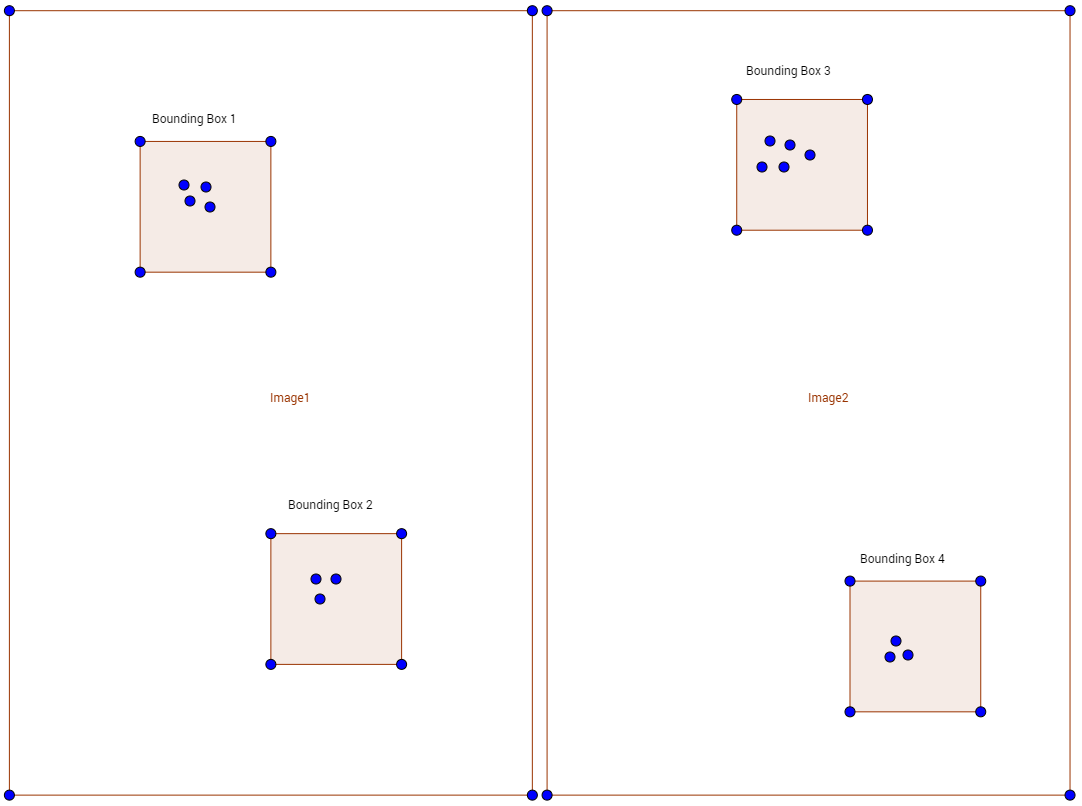
\includegraphics[width=\textwidth]{after_corner}

\subsection{RANSAC}

\end{document}